\documentclass[a4paper,10pt]{article}
\usepackage[utf8x]{inputenc}
\usepackage{natbib}
\usepackage{booktabs}
\usepackage[margin=0.9in]{geometry}
\usepackage{graphicx}
\usepackage{fancyvrb}
\usepackage{listings}
\usepackage{bm}
\usepackage{xcolor}
\usepackage{multirow}

\usepackage{hyperref}
\usepackage[capitalise]{cleveref}

\xdefinecolor{gray}{rgb}{0.4,0.4,0.4}
\xdefinecolor{blue}{RGB}{58,95,205}% R's royalblue3; #3A5FCD

\lstset{% setup listings
        language=R,% set programming language
        basicstyle=\ttfamily,% basic font style
        keywordstyle=\color{blue},% keyword style
        commentstyle=\color{gray},% comment style
        numberstyle=\scriptsize,% use small line numbers
        numbersep=10pt,% space between line numbers and code
        tabsize=3,% sizes of tabs
        showstringspaces=false,% do not replace spaces in strings by a certain character
        captionpos=b,% positioning of the caption below
        breaklines=true,% automatic line breaking
        escapeinside={(*}{*)},% escaping to LaTeX
        fancyvrb=false,% verbatim code is typset by listings
        extendedchars=false,% prohibit extended chars (chars of codes 128--255)
        literate={"}{{\texttt{"}}}1{<--}{{$\bm\leftarrow$}}1{<<-}{{$\bm\twoheadleftarrow$}}1
        {~}{{$\bm\sim$}}1{<=}{{$\bm\le$}}1{>=}{{$\bm\ge$}}1{!=}{{$\bm\neq$}}1{^}{{$^{\bm\wedge}$}}1,% item to replace, text, length of chars
        alsoletter={.<-},% becomes a letter
        alsoother={$},% becomes other
        otherkeywords={!=, ~, $, \&, \%/\%, \%*\%, \%\%, <-, <<-, /},% other keywords
        deletekeywords={c}% remove keywords
}


\graphicspath{{../figure/}}

%opening
\title{The performance of Iterative Proportional Fitting for spatial microsimulation: applying new tests to an old technique}
\author{Robin Lovelace}

\begin{document}

\maketitle

\begin{abstract}
Iterative Proportional Fitting (IPF)
is an established technique in Regional Science and
 has been used for a variety of purposes in the field, primary amongst these being 
the generation of small area microdata.  
The technique is mature, widely used and relatively straight-forward
yet there have been few studies focussed on evaluation of its performance. 
An additional research problem is the tendency of 
researchers to `start from scratch', resulting in a variety ad-hock implementations,
with little evidence of the merits of differing approaches.
Although IPF is well described mathematically, reproducible
examples of the algorithm, written in modern programming language, are rare in the academic literature.
These knowledge gaps mean that answers to methodological questions must be guessed:
Under what conditions can a `perfect' 
match be expected, and how can one test whether these conditions exist in the input datasets?  
How many iterations should be used for any given application? 
What is the impact of initial weights on the final results? 
And what impact will integerisation have on accuracy?  
This paper tackles such questions, using a systematic methodology 
based on publicly available code and input data. 
The results confirm IPF's status as robust and widely applicable 
method for combining areal and individual-level data and demonstrate the importance
of using various metrics of for determining its performace.
We conclude with an agenda for future tests and offer more general guidance on how the 
the method can be optimised to maximise its utility for future research.

Keywords: Iterative proportional fitting, spatial microsimulation, modelling

JEL Code: C
\end{abstract}

\section{Notes for authors}
Additonal papers to cite include:
\begin{itemize}
 \item \citet{harland2012}
\item \citet{Smith2009}
\item \citet{Cullinan2010}
\item 
\end{itemize}


\section{Introduction}
The aggregation of survey data has a long history in the social sciences. 
The most common form of 
aggregation conducted by national statistical agencies collecting data about citizens 
is 'flattening': converting data from `long' to `flat' form. This involves involves a) converting all 
variables into discrete categories (e.g.~an individual with an income of £13,000 per year
would be allocated to band of £10,000 to £15,000 per year), b) assigning a column to each category and c) assigning 
integer counts to cells in each column (Fig. 1). Each row in this aggregated form can 
represent the entire dataset or subsets thereof. (Geographical aggregation – one row 
per zone – is the most common form of aggregation, but any subsets, from social class, 
time period or other \emph{cross-tablulations} of the dataset can be used).

\subsection{IPF translates between `flat' and `long' data formats}
The main advantage of `flat' data is that it can summarise information about a very large number of individuals
in a small number of rows. Often, such flattened datasets are the only format in which 
statistical agencies make large datasets (e.g. the National Census) available, 
to save storage space, ease data analysis and ensure the anonymity and unidentifiability of survey respondents.
The main disadvantage is that the process of flattening is almost always associated with data loss: we do 
not know from a flat dataset if the hypothetical individual mentioned above earns \pounds10,000, \pounds15,000 or 
anywhere in between. Also, when flattening is associated with geographical aggregation, there is usually
a loss of geographical resolution: instead of knowing the person's full postcode from the full dataset, we 
may only be able to pin them down to a relatively large administrative zone such as a Local Authority in the UK context
in the flattened dataset. Finally, the cross-tabulations between the variables are generally during the process of 
flattening.
% make bullet points???

Both types of data representation are common in the physical sciences, although the raw data 
is usually available in long-form. In the social sciences, by contrast, the long format is often unavailable. 
As indicated above, this can be attributed to the long history of and confidentiality 
issues surrounding officially collected survey data. National Census datasets --- in which characteristics of 
every individual are recorded --- and some of the best datasets in social science are only available 
in flat form, however, posing major challenges to researchers in the sciences. 

A related long-standing research problem especially prevalent in geography and regional science
is the scale of analysis. There is often a trade-off between the quality and resolution 
of the data, which can result in a compromise between detail and accuracy of results 
\citep{ballas2003microsimulation-30-years}. A common scenario facing researchers investigating 
a spatial problem is being presented with two datasets: one long aspatial 
survey table where each row represents the characteristics of an individual --- such as
age, sex, employment status and income --- and another of `flat', geographically aggregated 
dataset containing count data for each category. 

As presented in Fig. 1, flat datasets are
are wider and shorter, containing multiple columns for each variable from the raw dataset.
The loss of information about the linkages between
the different variables is common, but not essential, in flat datasets. 
The solution to this problem, however, makes the flat datasets even more unwieldy, as
each new cross tabulation would add $nv1 \times nv2$ additional columns, where 
$nv1$ and $nv2$ are the number of discrete categories in contained in the variables to be
cross tabluted.\footnote{To 
provide a concrete example, a cross-tabulation 
of mode of travel to work by sex and social class would contain 540 (12 * 3 * 15) columns,
due to the number of categories present in each variable. 
Given that there are dozen of additional variables in any large census, this clearly become unwieldy.
} % figure???
The lack of cross tabulation is problematic because 
in many cases information about the linkages between different variables is needed to 
address policy-relevant questions. To pick one example related to 
policies targeted at skilled unemployed young adults: how many unemployed people 
reside in each geographical area who at the same time have a university degree, 
are female and over 25 years old? This question is impossible to answer with a 
geographically aggregated (flat) dataset.

\subsection{IPF in spatial microsimulation}
Spatial microsimulation tackles the afforementioned problems associated 
with the prevalent geographically aggregated flat data form by simulating
the individuals within each administrative zone. The most detailed output of this process of 
spatial microsimulation is `spatial microdata', a long table of individuals with 
associated attributes and weights for each zone (see \cref{t1} %???really
 for a simple example). 
Because these individuals correspond to observations in the survey dataset,
the spatial microdata generated in this way, of any size and complexity,
can be stored with only 3 columns: person identification number (ID), 
zone and weight. Weights are critical to spatial microdata generated in this way, as they 
determine how representative each individual is of each zone. Thus, an even more compact way 
of storing spatial microdata taken from a single dataset is as a `weight matrix' (table 2). 
% the same dataset can be stored using only two variables:  
% small area microdata 
% by combining the small area data with national survey data. The result of this process 
% of population synthesis (in its long % have we already defined long?
%  form --- it can also be represented in a flat table of counts)
%  is a table in which rows represent each 
% individual in the study region, with an additional column indicating the area of residence (Table 1).

Representing the data in this form offers a number of advantages (Clarke and Holm, 1987). These include:
\begin{itemize}
 \item The ability to investigate intra-zone variation (by analysing a the variable after subsetting 
a single area from the data frame),and inter-zone variation in the same dataset.
\item Cross-tabulations can be created for any combination of variables (e.g. age and employment status).
\item The presentation of continuous variables such as income as real numbers, 
rather than as categorical count data, in which there is always data loss.
\item The data is in a form that is ready to be passed into an individual-level model.
For example individual behaviour could simulate traffic, migration or the geographical distribution of future demand for healthcare.
\end{itemize}

% A potential downside of spatial microdata is that it can provide a misleading impression about the 
% quality and detail of the input data. It is important to remember that spatial microdata generated 
% in this way through spatial microsimulation are only as good as the constraint variables and the 
% extent to which the national dataset is representative of the zones in the study area.

These benefits have not gone unnoticed by the spatial modelling community.
Spatial microsimulation is now more than a methodology, and
can be considered as a research field in its
own right, with a growing body of literature, methods and results \citep{Tanton2013}.
In tandem with these methodological developments, a growing number of applied studies
has emerged to take advantage of the new possibilities opened up by such small area individual-level data,
with applications as diverse as the location of health services \citep{Tomintz2008} to the
analysis of commuting \citep{Lovelace2014-jtg}.
Various strategies for generating small area microdata are available,
as described in recent overviews on the subject \citep{Tanton2013, Ballas2013-4policy-analysis, Hermes2012a}.
However, it is not always clear which one is most appropriate,
as highlighted in the conclusions of a recent Reference Guide to spatial microsimulation
\citep[p~270]{Clarke2013-concs}:
``It would be desirable if the spatial microsimulation community were able to continue to
analyse which of the various reweighting/synthetic reconstruction techniques is most accurate
--- or to identify whether one approach is superior for some applications while another
approach is to be preferred for other applications''.

The longest-established and most straight-forward of these is Iterative Proportional Fitting (IPF), the performance of which is the subject of this paper...

\subsection{Applications}
\textbf{Dimitris and Eveline: please fill in this section}
Applications of IPF include using it ...

The application of greatest interest to regional scientists is as a method of 
spatial microsimulation: generating individual level data allocated to specific zones...
Papers that have used IPF in this context (or a subsitutable method such as simulated annealing)
have explored a range of regional economic problems that purely aggregate level analyses struggle to address.
These include:
\begin{itemize}
 \item using spatial microdata to analyses the wider impacts of major job losses
at the local level \citep{Ballas2006}.
\item an investigation into to local impacts of the marine sector in Ireland \citep{Morrissey2013a}
\item ...
\item ...
\end{itemize}

\section{IPF: theory and a worked example}
Iterative Proportional Fitting has a long history in Statistics and the social
sciences (especially in Economics and Geography).
In statistical language, IPF is used to estimate the values of internal
cells in a cross-tabulated table to fit known margins.
The method is also known as matrix raking or scaling,
biproportional fitting, RAS, and entropy maximising.
There are a number of texts discussing the method in a mathematical formal
way in some detail (for example \citealp{Mosteller1968, Fienberg1970, Pritchard2012}).
\citep{Birkin1988} provide a succinct presentation of the
mathematics of IPF and their work is the foundation of
the work presented here...% described in origin; rethink this...???

\subsection{IPF theory: a worked example} \label{s:theory}
In most modelling texts there is a strong precedence of theory over
application: the latter usually flows from the former. The location 
of this section after a description of the programming language
R is therefore a little unconventional but there is a logic to this order. 
Having demonstrated the power and flexibility of the programming language in
which the model is written, the next stage is to analyse the task to which it
is to be set. More importantly for reproducible research, this theory section
is illustrated with a simple worked example that culminates in
a question to the reader, to test his or her understanding.

IPF is a simple statistical procedure, ``in which cell counts in a contingency
table containing the sample observations are scaled to be consistent with
various externally given population marginals'' \citep{mcfadden2006testing}. In
other words, and in the context of \emph{spatial} microsimulation, IPF produces
maximum likelihood estimates for the frequency with which people appear in
different areas. The method is also known as `matrix raking' or the RAS
algorithm, 
% (\citealp{Birkin1988, Muller2010,Simpson2005, Kalantari2008, Jirousek1995})
 and has been described as one
particular instance of a more general procedure of `entropy maximisation'
\citep{Johnston1993, blien1998entropy}.
The mathematical properties of IPF
have been described in several papers
(\citealp{Bishop1975, Fienberg1970, Birkin1988}).
Illustrative examples of the procedure can be found in
\citet{Saito1992}, \citet{Wong1992}
and \citet{Norman1999a}. \citet{Wong1992} investigated the reliability of IPF
and evaluated the importance of different factors influencing the its
performance. Similar methodologies have since been employed by
\citet{Mitchell2000}, \citet{Williamson2002} and
Ballas et al.~\citeyearpar{Ballas2005c}
to investigate a wide range of phenomena.

To illustrate how IPF works in practice, a simplified example is described below.
This is a modified version of a simpler demonstration from
\citet{Ballas2005c}.\footnote{In \citet{Ballas2005c}
the interaction between the age and sex constraints are assumed to be known.
(Their equivalent of \cref{t:s2} contains data for every cell,
not question marks.) This results in IPF converging instantly.
However, in Census data, such cross-tabulation is
often absent, and IPF must converge over multiple constraints and
iterations. This latter scenario is assumed in the worked example below. Other
worked examples of the principles are provided in \citet[Appendix
3]{johnston1985geography} (for entropy maximisation), \citet{Norman1999a} and
\citet{Simpson2005} (using the proprietary statistical software SPSS).
}
Table \ref{t:w}  describes a
hypothetical microdataset comprising 5 individuals, who are defined by two
constraint variables, age and sex. Each has two categories.
Table \ref{t:s} contains aggregated data
for a hypothetical area, as it would be downloaded from census dissemination
portal Casweb. \Cref{t:s2} illustrates this table in a different form,
which shows our ignorance of interaction between age and sex.


\begin{table}[h]
\centering
\caption[A hypothetical input microdata set]{A
hypothetical input microdata set (the original
weights set to one). The bold value is used subsequently for
illustrative purposes.}
\begin{tabular}{llll}
\toprule
{Individual } & {Sex} & {Age-group} & {Weight} \\
\midrule
1 & Male & Over-50 & 1 \\
2 & Male & Over-50 & 1 \\
3 & {Male} & {Under-50} & \textbf{1} \\
4 & Female & Over-50 & 1 \\
5 & Female & Under-50 & 1 \\
\bottomrule
\end{tabular}
\label{t:w}
\end{table}
\vspace{1cm}


\begin{table}[htbp]
\centering
\caption{Hypothetical small area constraints data ($s$).}
\begin{tabular}{cllll}
\toprule
Constraint $\Rightarrow$ & \multicolumn{2}{c}{$i$}& \multicolumn{2}{c}{$j$}\\
Category $\Rightarrow$ & $i_1$ & $i_2$ & $j_1$ & $j_2$ \\
Area $\Downarrow$  & Under-50 & Over-50 &  Male & Female\\
1  & 8 & 4 & 6 & 6\\
\bottomrule
\end{tabular}
\label{t:s}
\end{table}
\vspace{1cm}

\begin{table}[htbp]
\centering
\caption[Small area constraints expressed as marginal totals]{Small
area constraints expressed as marginal totals, and the cell
values to be estimated.}
\begin{tabular}{cllll}\toprule
Marginal totals&  & \multicolumn{2}{c}{$j$} & \\
& Age/sex & Male & Female & T\\ \midrule
\multirow{2}{*}{$i$} & Under-50 & \textbf{?} & ? & 8\\
& Over-50 & ? & ? &4 \\
& T & 6 & 6 &12\\
\bottomrule
\end{tabular}
\label{t:s2}
\end{table}

Table \ref{t:m} presents the
hypothetical microdata in aggregated form,
that can be compared directly to Table \ref{t:s2}.

\begin{table}[htbp]
\centering
\caption[The aggregated results of the weighted
microdata set]{The aggregated results of the weighted
microdata set ($m(1)$).
Note, these values depend on the
weights allocated in Table \ref{t:w} and therefore
 change after each iteration}

\begin{tabular}{cllll}\toprule
Marginal totals&  & \multicolumn{2}{c}{$j$} & \\
& Age/sex & Male & Female & T\\ \midrule
\multirow{2}{*}{$i$} & Under-50 & \textbf{1} & 1 & 2\\
& Over-50 & 2 & 1 &3 \\
& T & 3 & 2 &5\\
\bottomrule
\end{tabular}
\label{t:m}
\end{table}

Using these data it is possible to readjust the weights of the hypothetical
individuals, so that their sum would add up to the totals given in Table
\ref{t:s2} (12). In particular, the weights can be readjusted by multiplying them by
the marginal totals, originally taken from
Table \ref{t:s} and then divided by the respective marginal total in \ref{t:m}.
Because the total for each small-area constraint is 12, this must be
done one constraint at a time. This
can be expressed, for a given area and a given constraint ($i$
or age in this case), as follows:

\begin{equation}
w(n+1)_{ij} = \frac{w(n)_{ij} \times sT_{i}}{mT(n)_{i}}
\label{eq:ipf}
\end{equation}
where $w(n+1)_{ij}$ is the new weight for individuals with characteristics $i$
(age, in this case), and $j$ (sex),  $w(n)_{ij}$ is the original
weight for individuals with these characteristics, $sT_{i}$ is element
marginal total of the small area constraint, $s$
(Table \ref{t:s}) and $mT(n)_{i}$ is the marginal total of category
$j$ of the aggregated results of the weighted
microdata, $m$ (Table \ref{t:m}). $n$ represents the iteration number.
Although the marginal totals of $s$ are known, its cell values
are unknown. Thus, IPF estimates the interaction (or cross-tabulation)
between constraint variables.
(Follow the emboldened values in the tables
to see how the new weight of individual 3 is calculated for the sex constraint.)
Table \ref{t:new-weights} illustrates the weights that result. Notice that the
sum of the weights is equal to the total population, from the constraint variables.

\begin{table}[htbp]
\centering
\caption{Reweighting the hypothetical microdataset in order to fit
Table \ref{t:s}.}
\begin{tabular}{lllll}
\toprule
{Individual} & {Sex} & {age-group} & {Weight} &
{New weight, w(2)} \\ \midrule
1 & Male & Over-50 & 1 & $1 \times 4/3 = \frac{4}{3}$ \\
2 & Male & Over-50 & 1 & $1 \times 4/3 = \frac{4}{3}$ \\
3 & Male & Under-50 & 1 & $\textbf{1} \times
\textbf{8}/\textbf{2} = 4$ \\
4 & Female & Over-50 & 1 & $1 \times 4/3 = \frac{4}{3}$ \\
5 & Female & Under-50 & 1 & $1 \times 8/2 = 4$ \\
\bottomrule
\end{tabular}
\label{t:new-weights}
\end{table}

After the individual level data have been re-aggregated (\cref{t:m2}),
the next stage is to repeat \cref{eq:ipf} for the age constraint to generate a
third set of weights, by replacing
the $i$ in $sT_{i}$ and $mT(n)_{i}$ with $j$ and incrementing the value of n:

\begin{equation}
w(3)_{ij} = \frac{w(2)_{ij} \times sT_{j}}{mT(2)_{j}}
\label{eq:ipf2}
\end{equation}

To test your understanding of IPF, apply \cref{eq:ipf2} to the information above
and that presented in \cref{t:m2}.
This should result in the following vector of new weights, for individuals 1 to 5:
\begin{equation}
%  w(3) = (\frac{6}{5}, \frac{?}{?}, \frac{18}{5}, \frac{?}{?}, \frac{9}{2})
  w(3) = (\frac{6}{5}, \frac{6}{5}, \frac{18}{5}, \frac{3}{2}, \frac{9}{2})
\end{equation}
As before, the sum of the weights is equal to the population of the area (12).
Notice also that after each iteration the fit between the marginal
totals of $m$ and $s$
improves. The total absolute error (TAE)
from $m(1)$ to $m(2)$ improves from
14 to 6 in \cref{t:m} and \cref{t:m2} above. TAE for $m(3)$ (not shown,
but calculated by aggregating $w(3)$) improves even more, to 1.3.
This number would eventually converge to 0 through subsequent
iterations, as there are no empty cells in the input microdataset;
a defining feature of IPF.


\begin{table}[htbp]
\centering
\caption[Aggregated results after constraining for age]{The
aggregated results of the weighted
microdata set after constraining for age ($m(2)$).
}

\begin{tabular}{cllll}\toprule
Marginal totals&  & \multicolumn{2}{c}{$i$} & \\
& Age/sex & Male & Female & T\\ \midrule
\multirow{2}{*}{$j$} & Under-50 & 4 & 4 & 8\\
& Over-50 & $\frac{8}{3}$ & $\frac{4}{3}$ & 4 \\
& T & $6\frac{2}{3}$ & 5$\frac{1}{3}$ & 12\\
\bottomrule
\end{tabular}
\label{t:m2}
\end{table}

The above process, when applied to more categories (e.g. socio-economic class)
and repeated iteratively until a satisfactory convergence occurs, results in a
series of weighted microdatasets, one for each of the small areas being
simulated. This allows for the estimation of variables whose values are not
known at the local level (e.g. income) \citep{Ballas2005c}. An issue
with the results of IPF (absent from combinatorial optimisation methods),
however, is that it results in non-integer weights: fractions of individuals
appear in simulated areas. As described in the introduction, this is not ideal
for certain applications. Integer weights allow the results of spatial
microsimulation to be further processed using dynamic microsimulation and agent
based modelling techniques \citep{Pritchard2012}.

% A key benefit from a policy perspective is that
% IPF and other spatial microsimultion techniques
% can provide estimation of variables whose values are not
% known at the local level (e.g. income).
Spatial microsimulation can also provide insight into the likely
distribution of individual level variables about which only
geographically aggregated statistics have been made available.
An issue
with the results of IPF (absent from combinatorial optimisation methods),
however, is that it results in non-integer weights: fractions of individuals
appear in simulated areas.

\subsection{Implementing IPF in R} \label{simplementing}
The above example is best undertaken by hand, probably with a pen and paper
to gain an understanding of IPF, before the process is automated for 
larger datasets. This section explains how the IPF
algorithm described above is implemented in R, using a slightly more
complex example
% This section is based on ``Spatial microsimulation in R: a
% beginner’s guide to iterative proportional fitting (IPF)'', a tutorial
% written to accompany a methods paper on integerisation
\citep{Lovelace2013-trs}.\footnote{This 
tutorial is available from Rpubs, a site dedicated
to publishing R analyses that are reproducible. It uses the RMarkdown
mark-up language, which enables R code to be run and presented within
documents. See http://rpubs.com/RobinLovelace/5089 \label{fnrpub} .
}

\section{Evaluation techniques}

To verify the integrity of any model, it is necessary to compare its outputs
with empirical observations or prior expectations gleaned from theory.
The same principles apply to spatial microsimulation, which can be evaluated using
both internal and \emph{external} validation methods \citep{Edwards2009}.
\emph{Internal validation} is the process whereby
the aggregate-level outputs of spatial microsimulation are compared with
the input constraint variables. Internal validation typically tackle such issues
as ``do the simulated populations in each area
microdata match the total populations implied by the constrain variables?''
and ``what is the level of correspondence between the cell values of different
attributes in the aggregate input data and the aggregated results of spatial microsimulation?''
As we shall see below, ideally we would hope for a perfect fit between the input
and output datasets during internal evaluation.
\emph{External validation} is the process whereby the variables that are
being estimated are compared to data from another source,
external to the estimation process, so the output dataset is compared with
another known dataset for those variables.
%... ?

This section outlines the evaluation techniques that are commonly used in the
field, with a strong focus on internal validation. The options for external
validation are heavily context dependent so must generally be decided on a
case-by-case basis, and are mentioned in passing with a focus on general principles
rather than specific advice. The methods are presented in ascending order of complexity
and roughly descending order of frequency of use, ranging from Pearson's coefficient of
correlation to entropy based measures. Before these methods are described, it is
worth stating the the purpose of this section is not to find the `best' evaluation metric:
each has advantages and disadvantages, the importance of which will vary depending on the
nature of the research. A final point is that the use of a variety of techniques in this paper
is of interest in itself. The high degree of correspondence between them (presented in \cref{cresults}),
suggests that researchers need only to present one or two metrics (but should
perhaps try more, for corroboration) to establish relative levels of goodness of fit between
different model configurations.

\subsection{Scatter plots and Pearson's coefficient of correlation}
A scatter plot of cell counts for each category for the original and simulated variables is
a basic but very useful preliminary diagnostic tool in spatial microsimulation
\citep{Ballas2005c,Edwards2009}.
In addition marking the points, depending on the
variable and category % have these been defined?
which they represent, can help identify which variables are particularly problematic,
aiding the process of improving faulty code (sometimes referred to as `debugging').

In these scatter plots each data point represents a single zone-category
combination (e.g. 16-25 year old female in zone 001), with the x axis value corresponding
to the number of individuals of that description in the input constraint table.
The y value corresponds to the
aggregated count of individuals in the same category in the aggregated
(flat) representation of the spatial microdata output from the model. % have we defined spatial microdata?
This stage can be conducted either before or after \emph{integerisation}
(more on this below). As taught in basic statistics courses, the closer the points to the
1:1 (45 degree, assuming the axes have the same scale) line, the better the fit.

Pearson's coefficient of correlation (henceforth Pearson's $r$) is a quantitative
indicator of how much deviation there is from this ideal 1:1 line. It varies from 0 to 1,
and in this context reveals how closely the simulated values fit the actual (census) data.
An $r$ value of 1 represents a perfect fit; an $r$ value close to zero suggests no correspondence
between then constraints and simulated outputs (i.e. that the model has failed).
We would expect to see very high coefficient of determination for
internal validation (the constraint) and strong
positive correlation between target variables that have been estimated and
external datasets (e.g. income).
% However, regression analysis does not give any information about the fit of the simulated data to the ‘ideal’ line (i.e. where y  =  x and the simulated data is the same as the actual data). Rather, R 2 expresses the fit of the data to the ‘best fit’ line through that data. That is, the coefficient of determination is providing information about precision, not accuracy (Edwards and Tanton, 2013).

% One way to do this is with a t test. With a spatial microsimulation model validation, the data are paired (given we are comparing simulated with actual data), thus an equal variance 2-tailed t test can be used to determine if there is any significant difference between the two datasets (i.e. simulated and actual). Thus, if the simulation is robust, we would expect to see no significant differences between the simulated and actual values for the input variables (and estimated/output variables, if known data are available). This enables the model accuracy to be assessed, as opposed to simply its precision.

\subsection{Standard error around identity (SEI)}
here SEI is the standard error around identity, y are the estimated values for
each area, y rel are the reliable estimates for each area from a census or other
data source and y rel is the mean estimate for all areas where reliable data are available.
This estimate has been used in validation by both Ballas and Tanton (see Ballas et al. 2007; Tanton et al. 2011).

\subsection{Total Absolute and Standardized Error (TAE and SAE)}
The SAE addresses this issue by using the population size as the denominator,
 but generally, authors seem to use total population, rather than the population
for that categorization of the variable, which may be deemed to understate the size
of the errors. Also, this measure does not provide any information on whether any
 differences are statistically significant (Edwards and Tanton, 2013).

\subsection{Z scores}
Here, the evaluation mainly takes place at the cell level (for a single constraint in a single area).
However, there should also be attention for the overall picture like spatial concentration.

% Spatial indicators etc??? Add equations to above methods soooon

\section{Input data}
Three input datasets form the basis of the scenarios tested in this paper,
`simple', `small-area' and `sheffield'. Each consists of a set of aggregate
constraints and corresponding individual-level survey tables.
The latter are anonymous and have been `scrambled' to enable their
publication on the internet. This enables the results to be replicated by others,
without breaching the user licenses of the data.
To this end, all the input data (and code) used to generate the results reported
in the paper are available online on the code-sharing site GitHub.
The simplest scenario consists of 6 zones which must be populated by a
sample survey dataset of only five individuals, constrained by two variables (age and sex).
This scenario is purely hypothetical and is used to represent the IPF procedure
and the tests in the simplest possible terms. Its small size allows the entirety
of the input data to be viewed in a couple of tables that fit on a single page
(see \cref{t1} and \cref{t2}). As with all data used in this paper, these tables can be
viewed and downloaded online.

\begin{table}[htbp]
\caption{Individual-level data for the simple scenario. The file, `vailable from the GitHub in the folder 
`\href{https://github.com/Robinlovelace/IPF-performance-testing/tree/master/input-data/small-area-eg}{input-data}'} % where???
\begin{center}
\begin{tabular}{rrl}
\toprule
\multicolumn{1}{l}{Id} & \multicolumn{1}{l}{Age} & Sex \\
\midrule
1 & 59 & m \\
2 & 54 & m \\
3 & 35 & m \\
4 & 73 & f \\
5 & 49 & f \\
\bottomrule
\end{tabular}
\end{center}
\label{t1}
\end{table}

\begin{table}[htbp]
\caption{Geographically aggregated constraint variables for the simple scenario, also available online}
\begin{center}
\begin{tabular}{rrrrr}
\toprule
\multicolumn{1}{l}{} & \multicolumn{2}{c}{Age constraint} & \multicolumn{2}{c}{Sex constraint} \\
\multicolumn{1}{l}{Zone} & \multicolumn{1}{c}{16--49} & \multicolumn{1}{c}{50+} & \multicolumn{1}{c}{m} & \multicolumn{1}{c}{f} \\
\midrule
1 & 8 & 4 & 6 & 6 \\
2 & 2 & 8 & 4 & 6 \\
3 & 7 & 4 & 3 & 8 \\
4 & 5 & 4 & 7 & 2 \\
5 & 7 & 3 & 6 & 4 \\
6 & 5 & 3 & 2 & 6 \\
\bottomrule
\end{tabular}
\end{center}
\label{t2}
\end{table}

The next smallest input dataset, and the most commonly used scenario in the paper, 
is `small-area'. The area constraints consist of 24 Output Areas (the smallest 
administrative geographical unit in the UK), with an average population of 184 people aged over 16. 
Three files describe the number of hours worked, the marital status and the tenancy of these 
individuals (although tenancy in fact counts houses, not people): the files can be accessed 
from the hyperlinks embedded in digital versions of the previous sentence. 
% Add these
A sample of these constraint variables is presented in \cref{t3} below. % aren't we putting ind. data 1st?

\begin{table}[htbp]
\caption{Sample of constraint variables from the first 5 rows of the small-area-eg input dataset.}
\begin{center}
\begin{tabular}{rrrrr}
\toprule
\bottomrule
\end{tabular}
\end{center}
\label{t3}
\end{table}

The individual-level table that compliments these geographically aggregated count constraints 
is taken from Understanding Society wave 1. These have been randomized to ensure anonymity
but they are still roughly representative of real data. The table consists of 1768 rows of 
data and is stored in R’s own space-efficient filetype (see ``ind.RData'', which must be opened in 
R to be viewed properly). As shown in \cref{t4} below, this consists of the same 3 
constraint variables as provided in \cref{t3} but at aggregate level, in addition to one 
`target variable': monthly pre-tax income in pounds. 

\begin{table}[htbp]
\caption{Randomly selected sample of 5 individuals taken from the individual-level dataset.}
\begin{center}
\begin{tabular}{rrrrr}
\toprule
\bottomrule
\end{tabular}
\end{center}
\label{t4}
\end{table}

... More here on loading-up this data.

\section{Method: model experiments}
\subsection{Baseline scenarios}
In order to perform a wide range of model experiments, 
in which only one factor is altered at a time, it was necessary 
to clearly define baseline scenarios. These are model runs with sensible 
defaults, which can be referred back to as a reference point and re-used at 
any point in the future. The baseline ‘simple’ scenario consists of 3 iterations, 
leading to a total of 6 constraint-iteration permutations. The results of simplest 
baseline scenario are shown in \cref{tblresults1}. The results show that the model 
fit improves after every iteration and every constraint in every measure of model 
fit (except `p5', which reaches zero in the second iteration) --- $pcor$ continues to improve, 
even though the printed value, to 6 decimal places, is indistinguishable from 1 after two complete iterations.

\begin{table}[htbp]
\caption{Results for the baseline `simple' scenario. Generated through by the ‘analysis’ script, and available as a .csv file online.}
\begin{center}
\begin{tabular}{rrrrr}
\toprule
\bottomrule
\end{tabular}
\end{center}
\label{tblresults1}
\end{table}

The baseline `small-area' scenario consists of three
 iterations of IPF, in which all three constraints were 
used. The results for all 9 constraint-iteration permutations 
of this baseline scenario are illustrated in \cref{fipfinac} and %??? ref
in the online `measures' table. These results show that IPF successfully 
brings the simulated cell counts in-line with the census after each constraint 
is applied and that the fit improves with each iteration (only two iterations are 
shown here, as the fit improves very little beyond two, and to avoid clutter).

\begin{figure}
 \begin{center}
  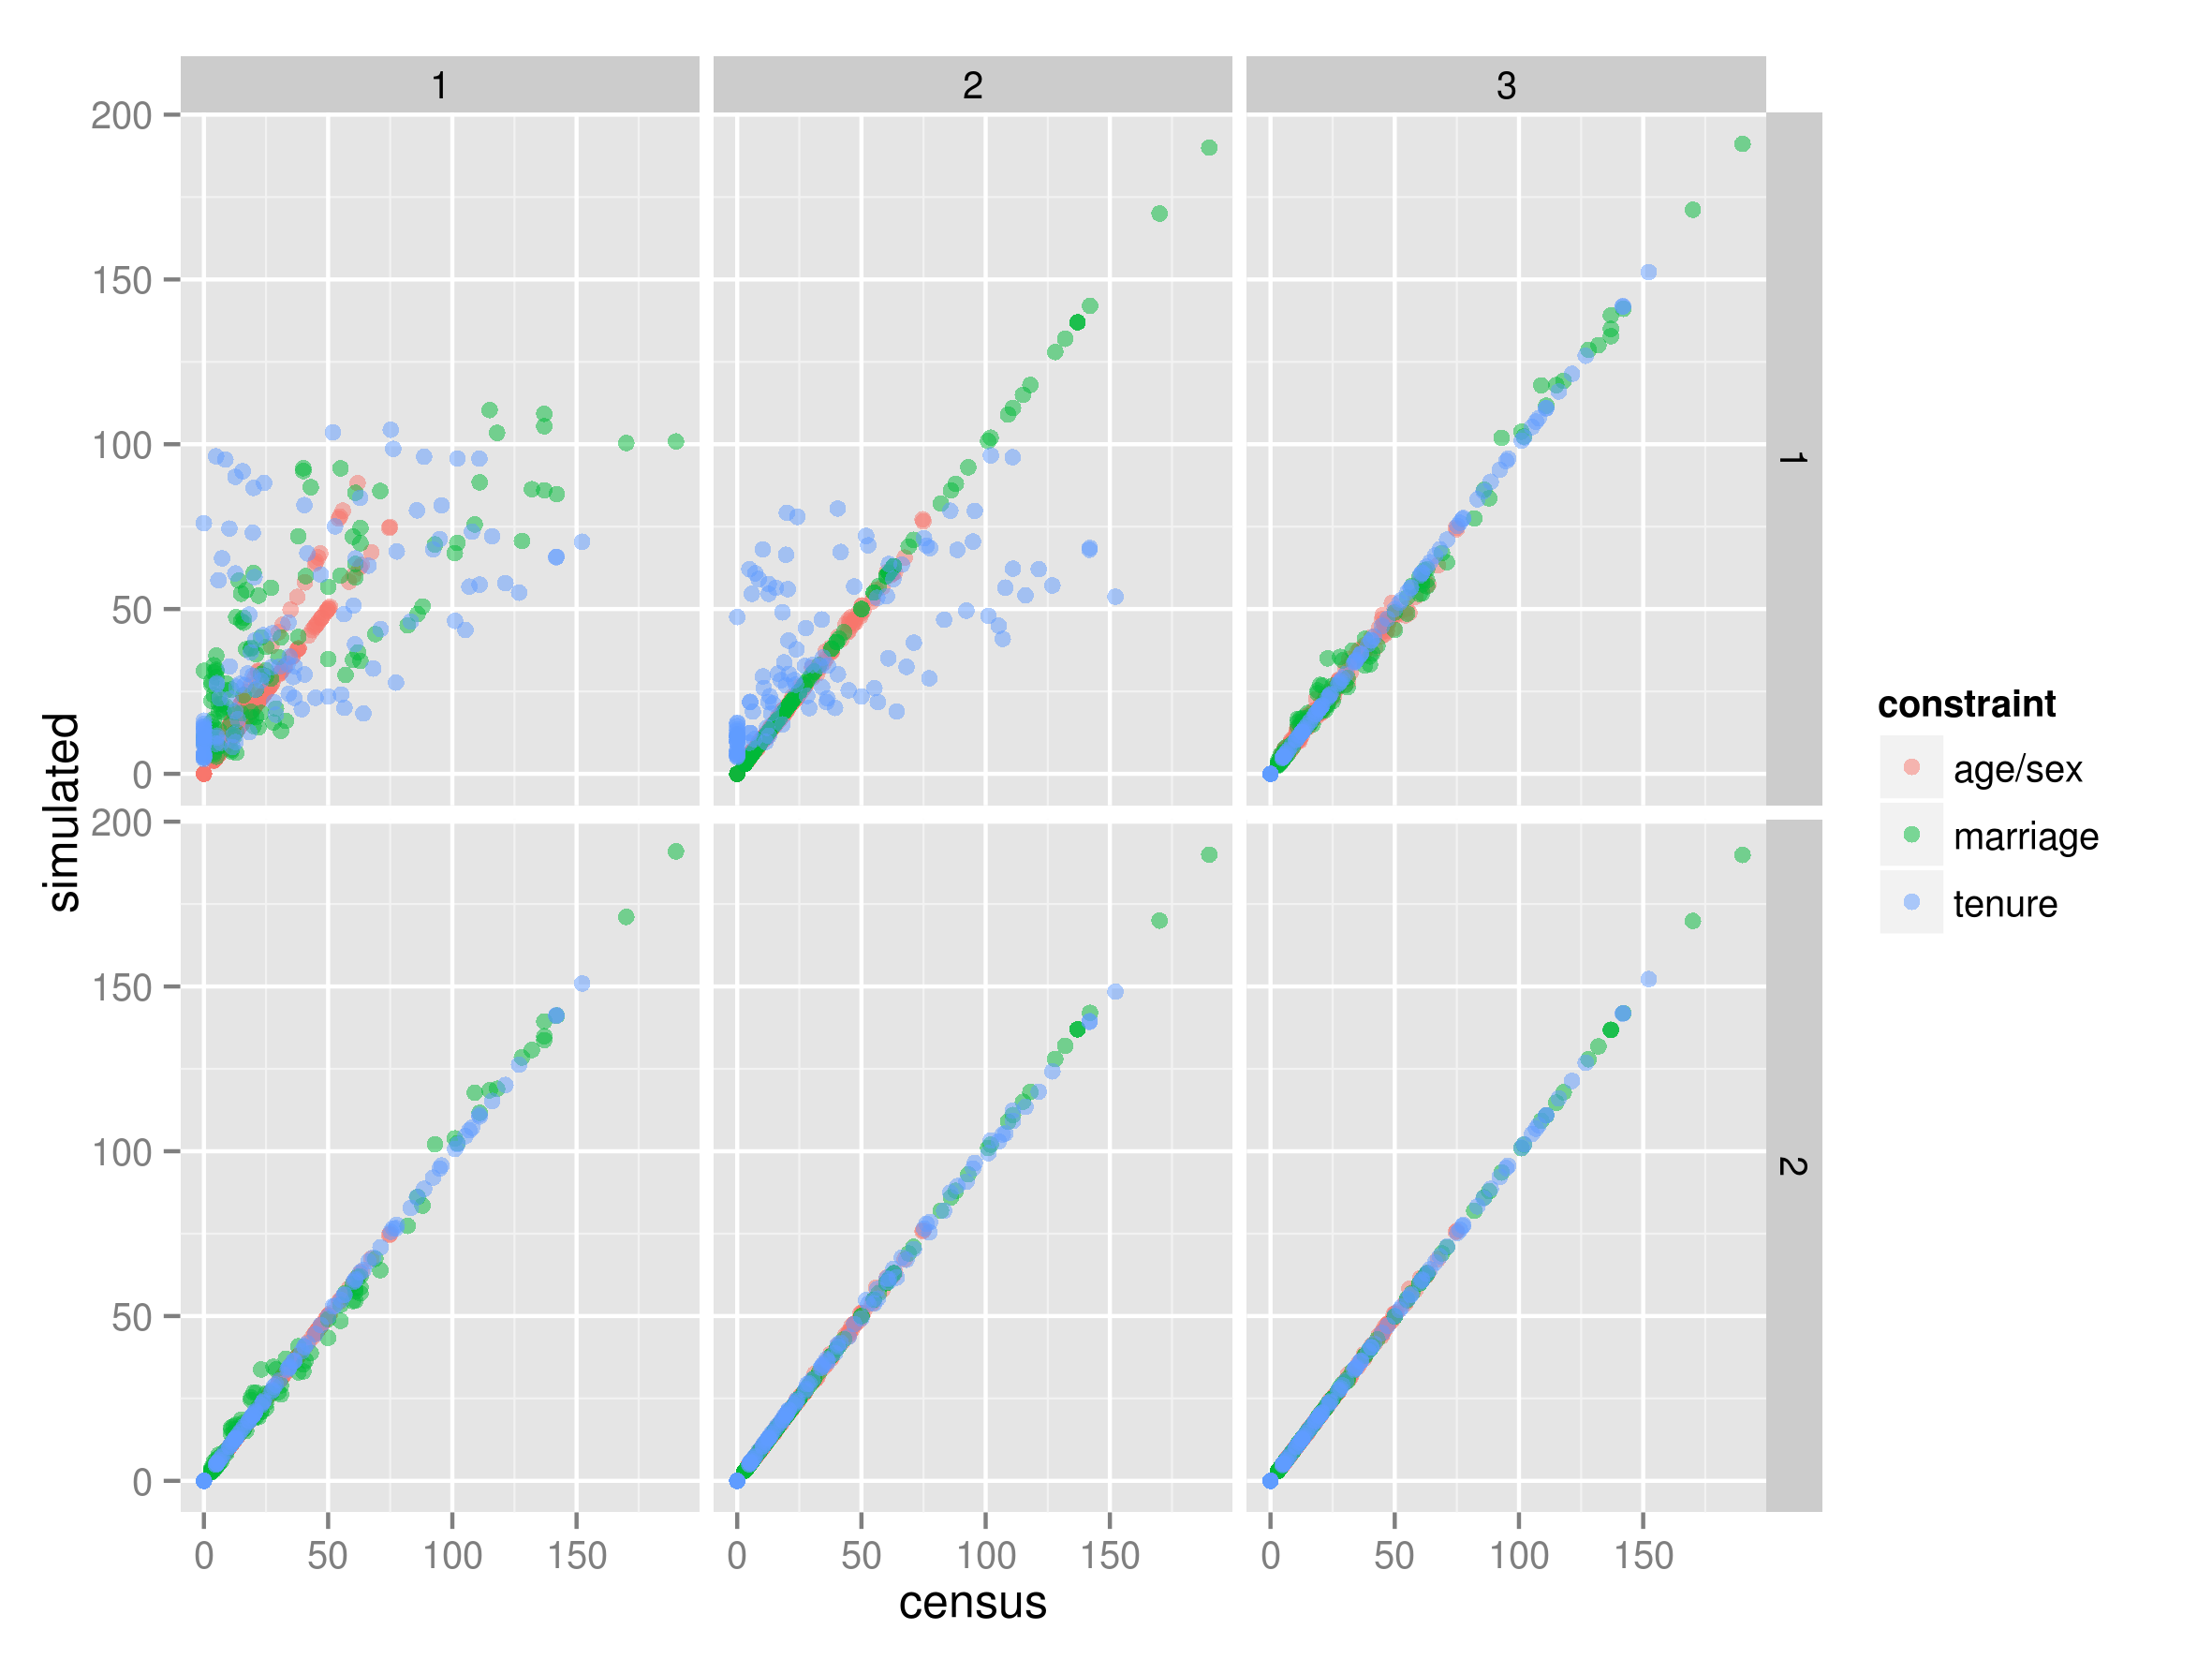
\includegraphics[width=12cm]{ipfinac}
 \end{center}
\caption{IPF in action: simulated vs census zone counts for the small-area baseline scenario after each constraint (columns) and iteration (rows).}
\label{fipfinac}
\end{figure}

The baseline `Sheffield' scenario consists of the same basic set-up, 
but with 4 constraints. As before, the results show convergence 
towards better model fit, although the fit does not always improve 
from one constraint to the next (see the online `measures' table). % online???

\subsection{Constraints and iterations}
These were the simplest model experiments, requiring only
 the reporting of iterations that had already taken place,
 and re-arrangement of the IPF code such that constraints
 were applied in a different order than before. 
The re-ordered code for the `small-area' scenario, 
for example can be seen in the script `etsim-reordered' online.

\subsection{Initial weights}
The impact of initial weights was tested in two ways: first, the impact
 of changing a sample of one or more initial weight values by a set 
amount was explored. Second, the impact of of the size of the initial 
weights was tested, by running the same model experiment several times, 
but with incrementally larger initial weights applied to a pre-determined set of individuals.

\subsection{Empty cells} 
Empty cells refer to cross-tabulations of individual-level 
attributes that are not represented by any single individual 
in the survey input data. An example of this would be if no female 
in the 16 to 49 year age bracket were present in \cref{t1}. 
The method used to find-out if empty cells exist is to first 
select only individuals with unique characteristics 
(in the narrow terms of the constraint variables --- of course every survey individual is unique). 
The column totals of the categorical (binary, 0 or 1) form of this dataset are compared: 
any categories with fewer than expected totals have missing cells. 

Once the presence of empty cells is determined in the baseline scenarios, the next 
stage is to add or subtract empty cells by adding or subtracting individuals to the 
input data. After these changes were made, the baseline scenarios were run as before.

In the ‘simple’ scenario, this simply involves removing a single individual from the 
input data, which equates to deleting a single line of code (see `etsim-empty'). %??? online 
The question of which unique individual to remove is solved by random sampling. 

\subsection{Integerisation}
This was the next variable that was altered, 
following \citep{}. In the simplest scenario, the 
initial weight of a single individual was altered 
repeatedly, in a controlled manner. The code enabling this model experiment 
is contained in the folder `small-area-weights' (see `etsim.R'). 
The number of different initial weights can be controlled by the 
parameter `num.ws' which is set to 5 as an arbitrary default.
Initial weights are set to k, a vector of length `num.ws' which
are by default set as a function of `u' which is in term
defined as the sequence 1:num.ws:

\begin{lstlisting}
k <- u/5 + 0.5 # initial weight of sample individuals for testing 
\end{lstlisting}

In this case the resultant weights are set to
 0.7, 0.9, 1.1, 1.3 and 1.5 for each model experiment. 
For factors of one million, for example, 
the above would be replaced by \lstinline !k <- u * 10^6 yrm!. 
To observe the impacts of altering the weights in this way
the usual tests of model fit were conducted. In addition,
the capacity of initial weights to influence an individual's 
final weight/probability of selection was tested by tracing its
weight into the future after each successive constraint and iteration. 
This enabled plotting original vs simulated weights under a 
range of conditions (\cref{cresults}).
  

\section{Results}
\label{cresults}

\subsection{Baseline scenarios}
As expected from \cref{fipfinac} above, the correlation of 
the baseline scenario improves over time, with each constraint 
and from one iteration to the next. Through the course of the first 
iteration, the correlation improves from 0.67 (the correlation between 
the frequencies of variables in the survey dataset and their frequencies 
in the census dataset, for each zone) to 0.9981. As illustrated in \cref{fnconscor}, 
the marginal improvement reduces from one iteration to the next: 
at the end of iteration 2, the correlation has improved to 0.999978.   

\begin{figure}
 \begin{center}
  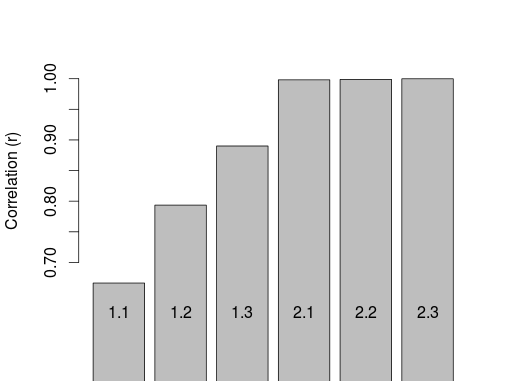
\includegraphics[width=6cm]{corr-baseline}
 \end{center}
\caption{Improvement in goodness of fit with additional constraints and iterations, 
as illustrated by $r$ values.}
\label{fnconscor}
\end{figure}

\subsection{Constraints and iterations}
As illustrated above, the number of iterations 
required to reach a very close fit between the census
 and simulated data is very low, with rapid reductions in
 the marginal accuracy return on additional computing power.
 After four iterations, the result in R is indistinguishable from 1,
 with its default accuracy of 7 decimal places. 
The decay in the rate of improvement with additional 
iterations and constraints was found to super-exponential. 

\subsection{Initial weights}
It was found that initial weights had little impact on the overall simulation. 
Taking the simplest case, a random individual (id = 228) was selected from the 
`small area' data and his/her initial weight was set to 2 
(instead of the default of 1). The impact of this change on the individual's 
simulated weight decayed rapidly, tending to zero after only 5 iterations in the small-area scenario. 
It was found that altered initial weights affect the simulated weights of all other individuals; 
this is illustrated in \cref{ficweight}, which shows the impact on individual 228 and a randomly selected 
individual whose initial weight was not altered, for all areas.

\begin{figure}
 \begin{center}
  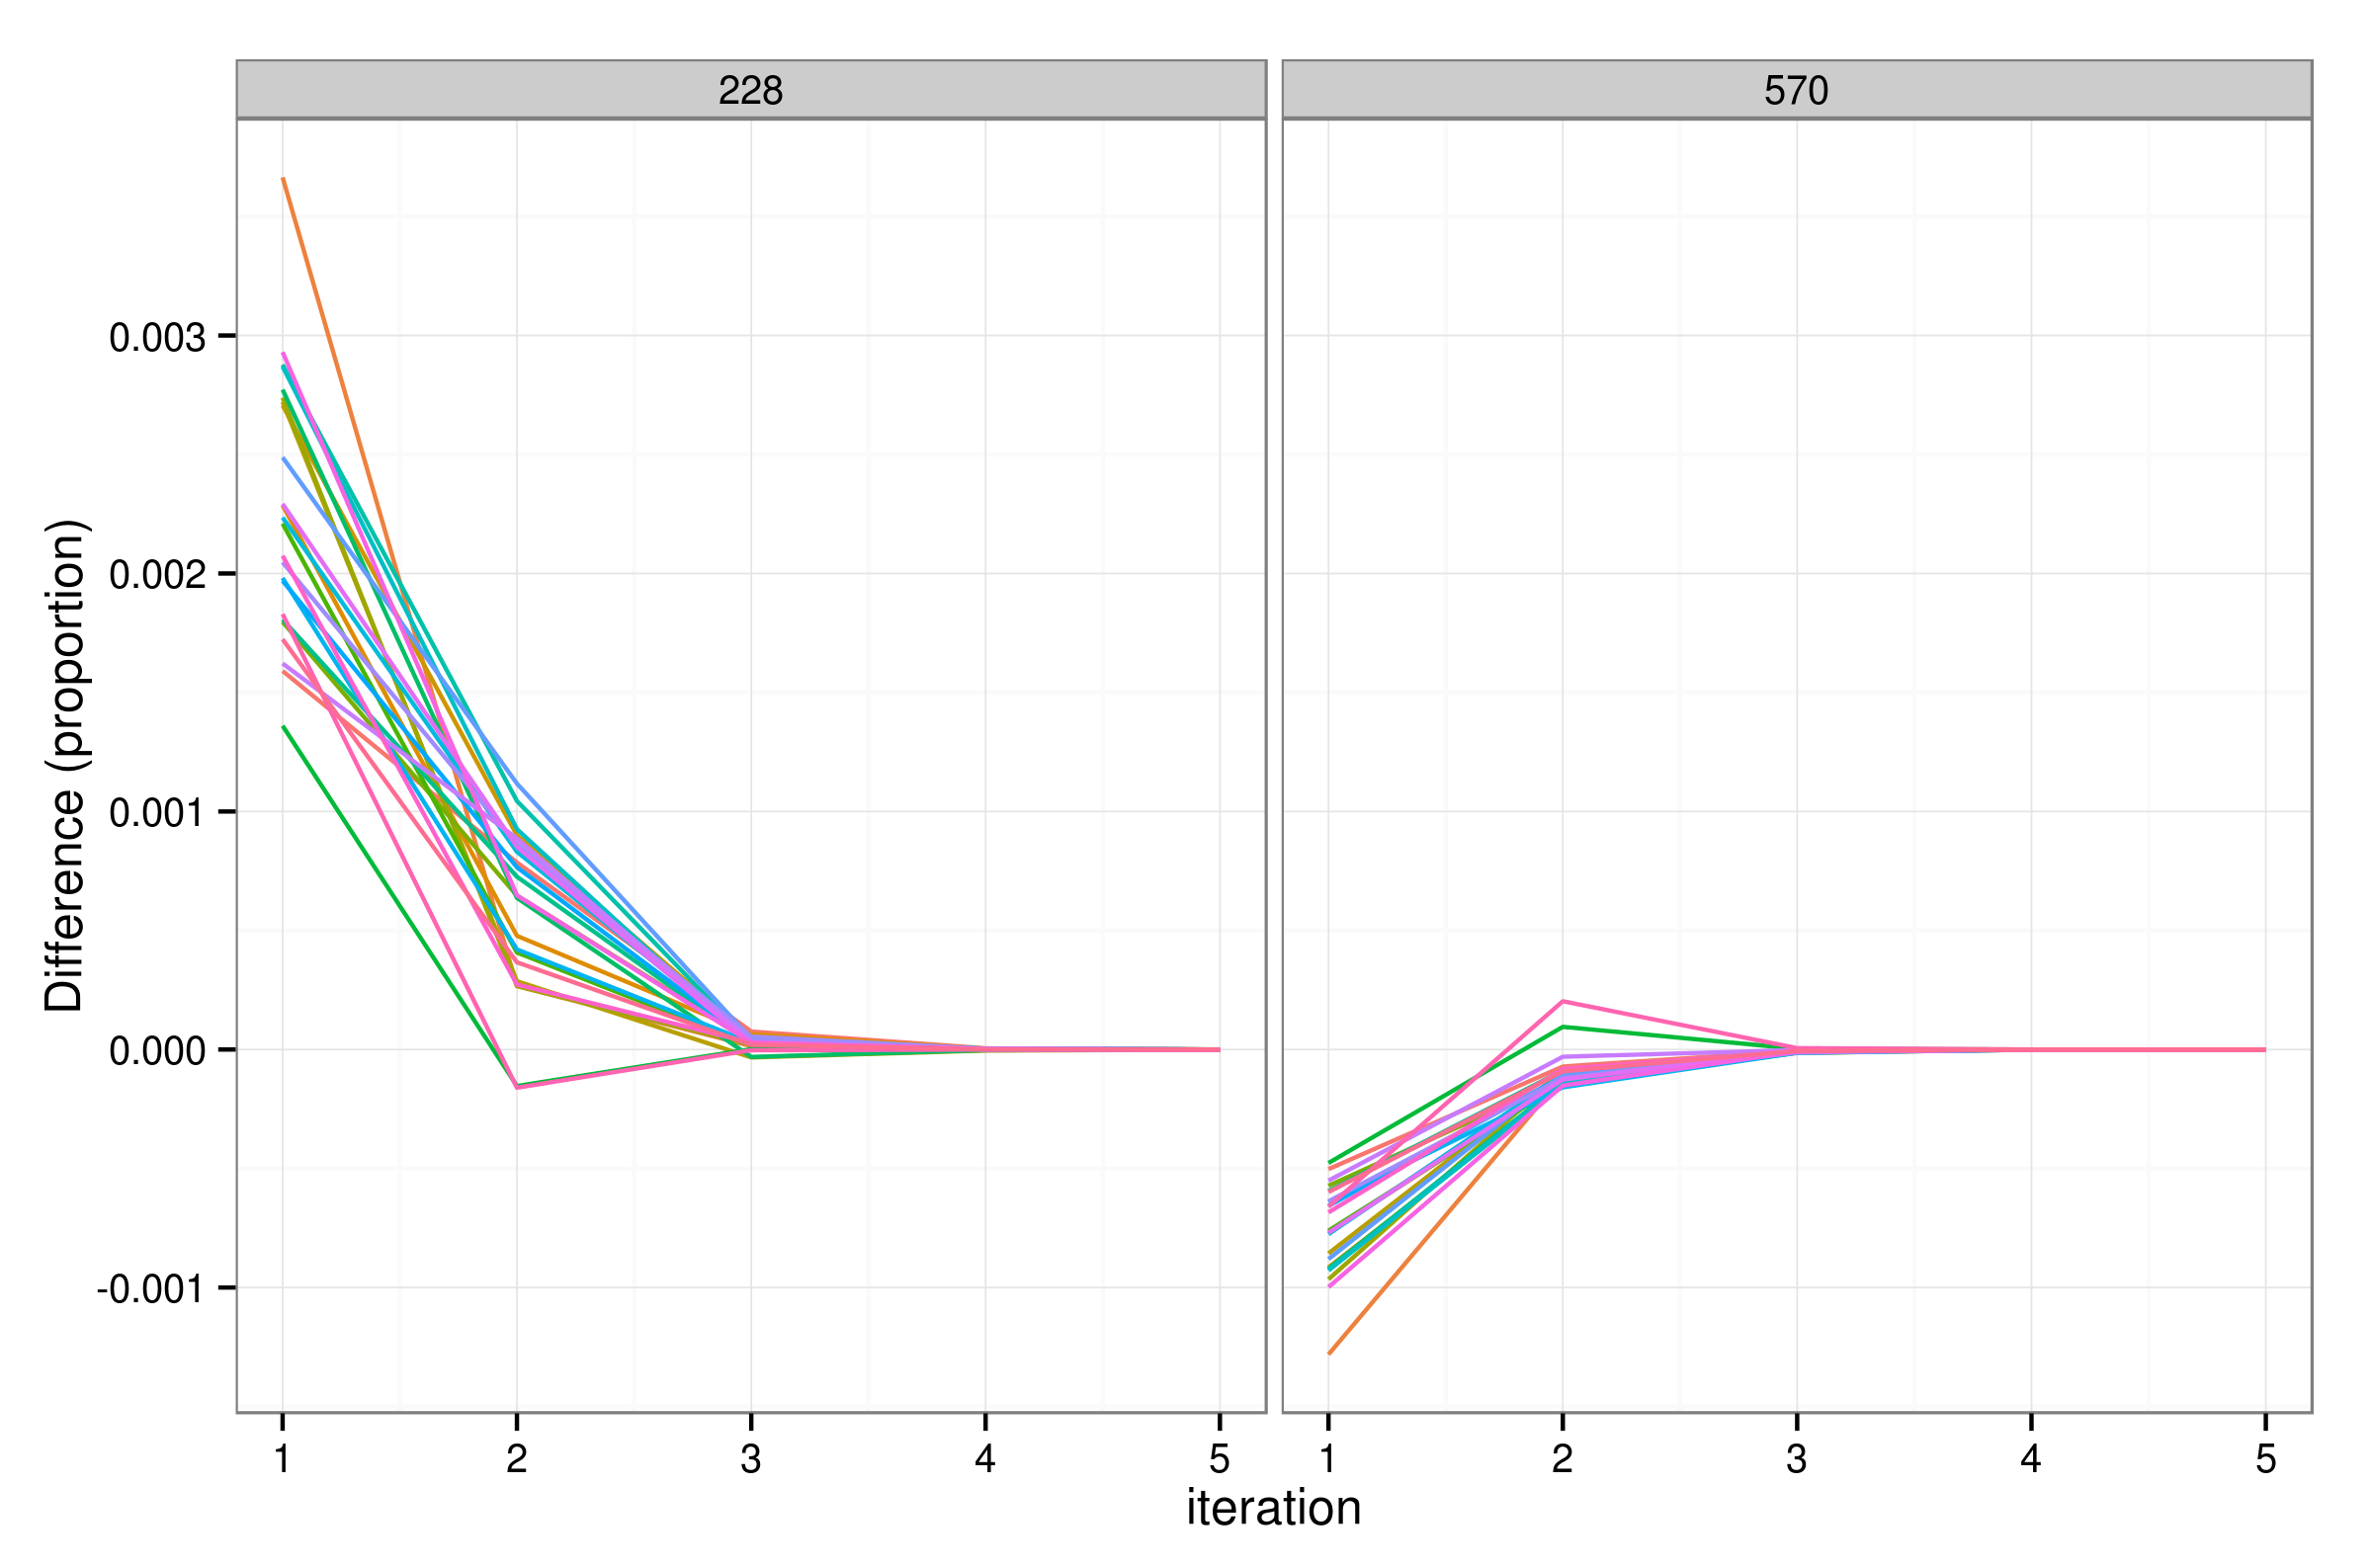
\includegraphics[width=12cm]{weight-1-5-its}
 \end{center}
\caption{The impact of changing the initial weight of individual 228 on the simulated weights of two individuals after 5 iterations. Each of the 24 coloured lines represents a single zone.}
\label{ficweight}
\end{figure}

\cref{ficweight} shows that changing initial weights 
for individuals has a limited impact on the results that
 tends to zero from one iteration to the next. 
After iteration one the impact of a 100\% increase in the initial weight 
of individual 228 had reduced to 0.3\%; after 3 iterations the impact was negligible. 
The same pattern can be observed in the control individual 570, 
although the impact is smaller and in the reverse direction. 
The same pattern can be observed for other individuals, by altering the `analysis.min'.

To analyse the impacts of changing the initial weights of multiple 
individuals, the same experiment was conducted, but this time the initial weights were
applied to the first five individuals. The results are illustrated in \cref{finweight},
which shows the relationship between initial and final weights for the first two individuals
and another two individuals 
(randomly selected to show the impact of altering weights on other individual weights). 

\begin{figure}
 \begin{center}
  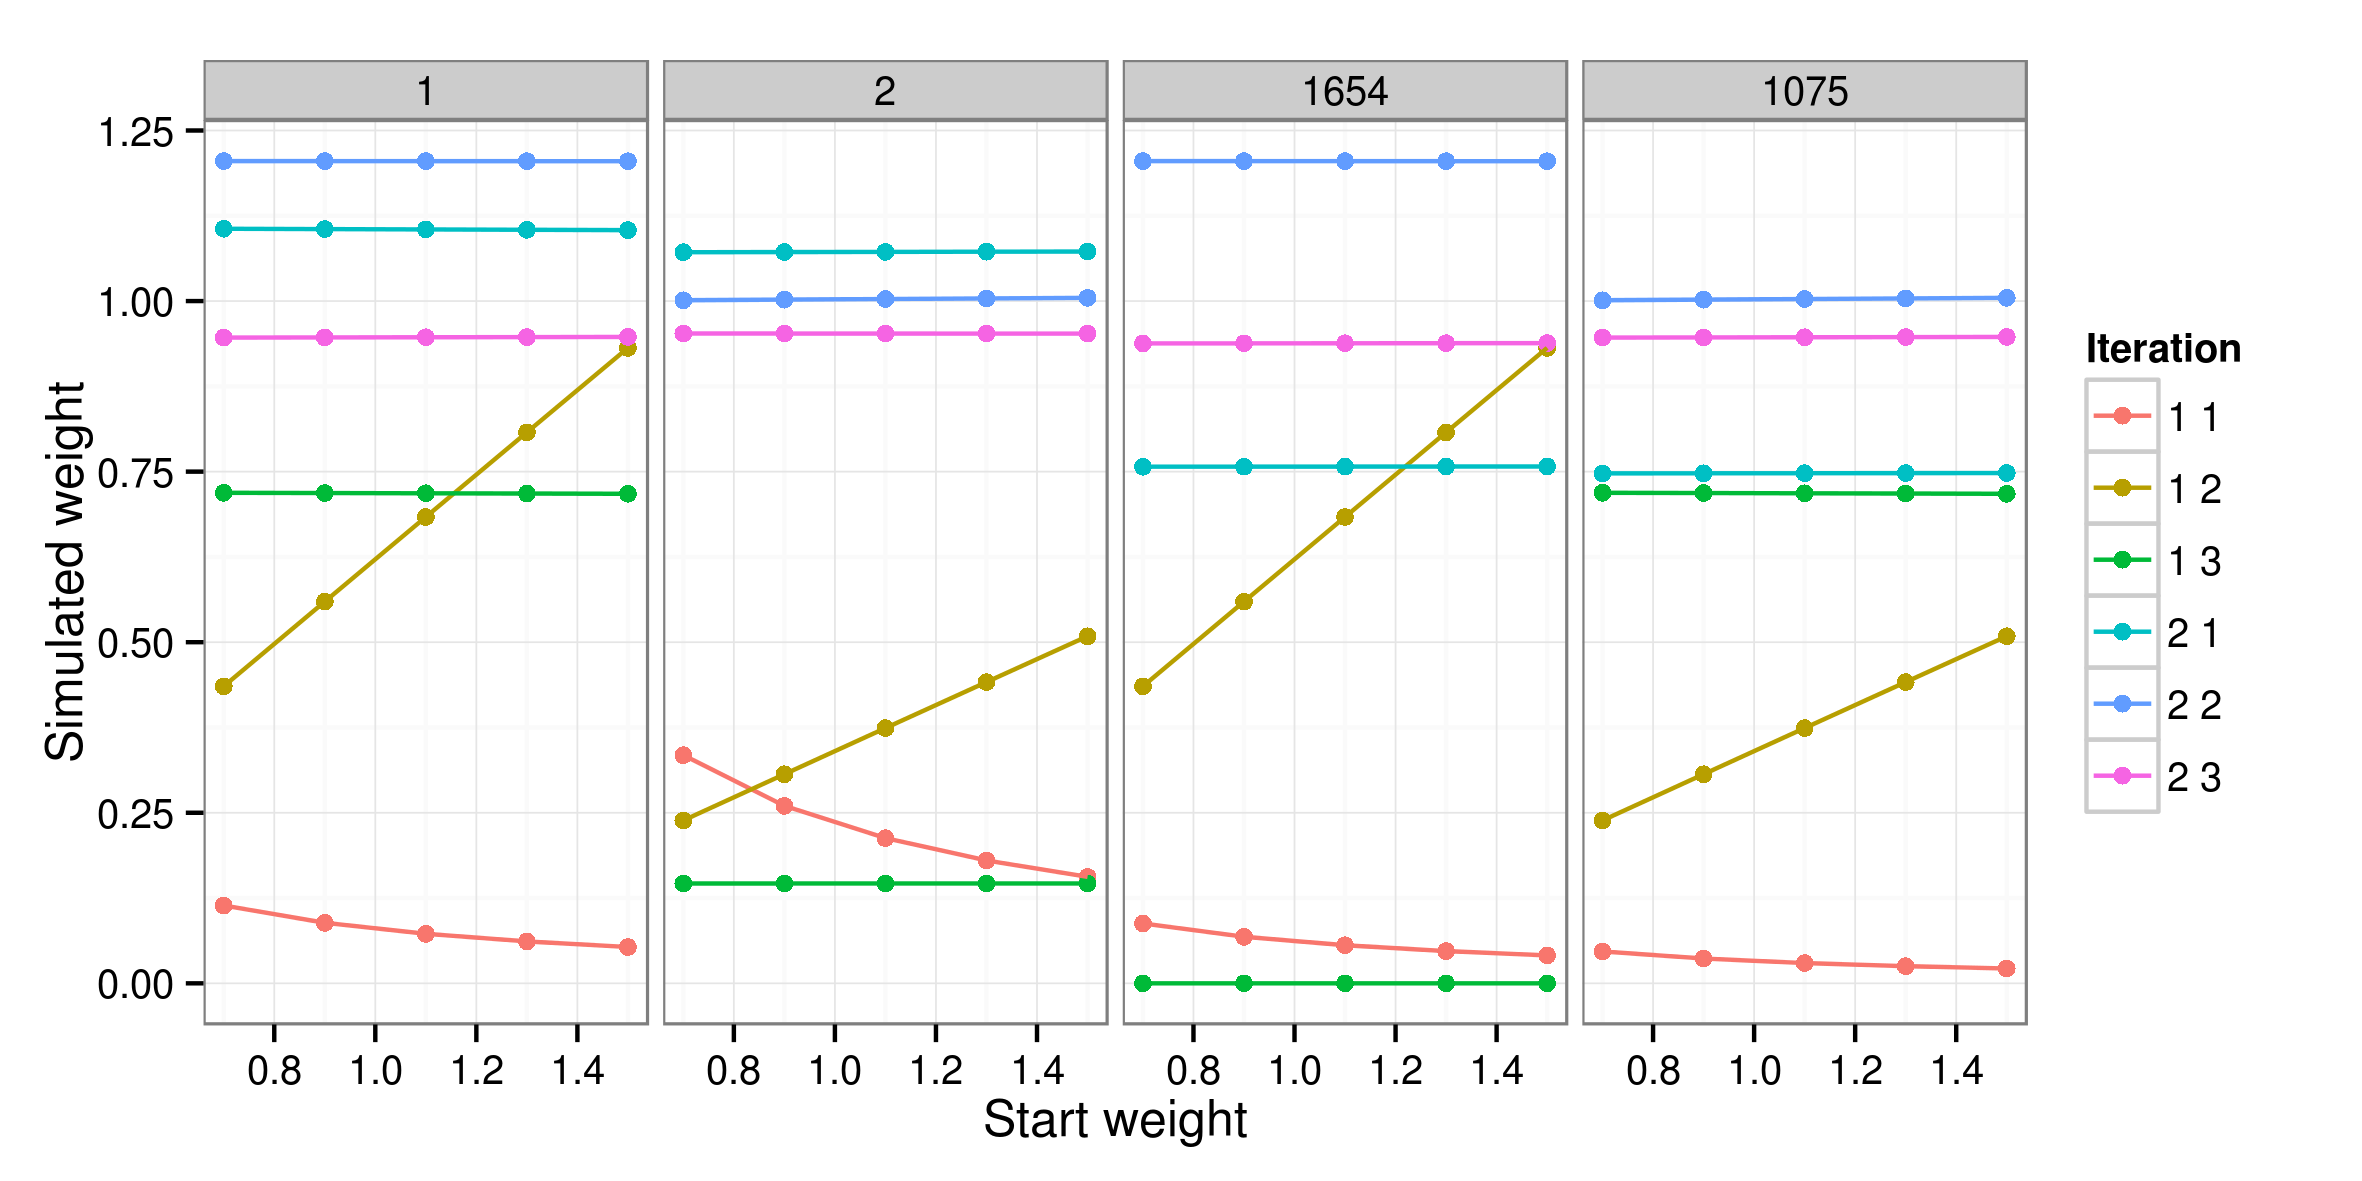
\includegraphics[width=12cm]{weights-exp-54nice2}
 \end{center}
\caption{Initial vs simulated weight of four individuals for a single area (zone 1).}
\label{finweight}
\end{figure}

\cref{finweight} shows that the vast majority of the impact of altered starting weights occurs in iteration-constraint
combinations 1.1 and 1.2, before a complete iteration has even occurred. 
After that, the initial weights continue to have an influence, of a magnitude that cannot be 
seen. For individual 1, the impact of a 53\% difference in initial weights (from 0.7 to 1.5) shrinks to 
2.0\% by iteration 1.3 and to 1.1\% by iteration 2.3. 

These results suggest that initial weights have a limited impact on the results of IPF, that declines rapidly with each iteration. 

\subsection{Empty cells}
\subsection{Integerisation}


\section{Conclusions}


\bibliographystyle{model2-names.bst}
\bibliography{/nfs/foe-fs-01_users/georl/Documents/Microsimulation.bib, /home/robin/Documents/powerstarrefs/Microsimulation.bib}
%/nfs/foe-fs-01_users/georl/repos/IPF-performance-testing/paper/ipflib.bib  desktop.bib,
% /home/robin/Documents/powerstarrefs/Microsimulation.bib


\end{document}